\documentclass[hidelinks,12pt]{article}
\usepackage[left=0.25cm,top=1cm,right=0.25cm,bottom=1cm]{geometry}
%\usepackage[landscape]{geometry}
\textwidth = 20cm
\hoffset = -1cm
\usepackage[utf8]{inputenc}
\usepackage[spanish,es-tabla]{babel}
\usepackage[autostyle,spanish=mexican]{csquotes}
\usepackage[tbtags]{amsmath}
\usepackage{nccmath}
\usepackage{amsthm}
\usepackage{amssymb}
\usepackage{mathrsfs}
\usepackage{graphicx}
\usepackage{subfig}
\usepackage{standalone}
\usepackage[outdir=./Imagenes/]{epstopdf}
\usepackage{siunitx}
\usepackage{physics}
\usepackage{color}
\usepackage{float}
\usepackage{hyperref}
\usepackage{multicol}
%\usepackage{milista}
\usepackage{anyfontsize}
\usepackage{anysize}
%\usepackage{enumerate}
\usepackage[shortlabels]{enumitem}
\usepackage{capt-of}
\usepackage{bm}
\usepackage{relsize}
\usepackage{placeins}
\usepackage{empheq}
\usepackage{cancel}
\usepackage{wrapfig}
\usepackage[flushleft]{threeparttable}
\usepackage{makecell}
\usepackage{fancyhdr}
\usepackage{tikz}
\usepackage{bigints}
\usepackage{scalerel}
\usepackage{pgfplots}
\usepackage{pdflscape}
\pgfplotsset{compat=1.16}
\spanishdecimal{.}
\renewcommand{\baselinestretch}{1.5} 
\renewcommand\labelenumii{\theenumi.{\arabic{enumii}})}
\newcommand{\ptilde}[1]{\ensuremath{{#1}^{\prime}}}
\newcommand{\stilde}[1]{\ensuremath{{#1}^{\prime \prime}}}
\newcommand{\ttilde}[1]{\ensuremath{{#1}^{\prime \prime \prime}}}
\newcommand{\ntilde}[2]{\ensuremath{{#1}^{(#2)}}}

\newtheorem{defi}{{\it Definición}}[section]
\newtheorem{teo}{{\it Teorema}}[section]
\newtheorem{ejemplo}{{\it Ejemplo}}[section]
\newtheorem{propiedad}{{\it Propiedad}}[section]
\newtheorem{lema}{{\it Lema}}[section]
\newtheorem{cor}{Corolario}
\newtheorem{ejer}{Ejercicio}[section]

\newlist{milista}{enumerate}{2}
\setlist[milista,1]{label=\arabic*)}
\setlist[milista,2]{label=\arabic{milistai}.\arabic*)}
\newlength{\depthofsumsign}
\setlength{\depthofsumsign}{\depthof{$\sum$}}
\newcommand{\nsum}[1][1.4]{% only for \displaystyle
    \mathop{%
        \raisebox
            {-#1\depthofsumsign+1\depthofsumsign}
            {\scalebox
                {#1}
                {$\displaystyle\sum$}%
            }
    }
}
\def\scaleint#1{\vcenter{\hbox{\scaleto[3ex]{\displaystyle\int}{#1}}}}
\def\bs{\mkern-12mu}


\usetikzlibrary{babel}
\setlength{\tabcolsep}{12pt}
\title{Tensores \\ \large{Material de consulta previo}\vspace{-3ex}}
\author{M. en C. Gustavo Contreras Mayén}
\date{ }
\begin{document}
\vspace{-4cm}
\maketitle
\fontsize{14}{14}\selectfont
\tableofcontents
\newpage


%Ref. Heinbockel (1996) Introduction to tensor calculus and continuum mechanics.
\section{Concepto de tensores.}

Para los vectores unitarios ortogonales independientes $\vu{e}_{1}, \vu{e}_2, \vu{e}_{3}$ (vectores base), podemos escribir cualquier vector $\va{A}$ como:
\begin{align*}
\va{A} = A_{1} \, \vu{e}_{1} + A_{2} \, \vu{e}_{2} + A_{3} \, \vu{e}_{3}
\end{align*}
donde $(A_{1}, A_{2}, A_{3})$ son las coordenadas del vector $\va{A}$ relativas a los vectores base elegidos. Estas componentes son la proyección de $\va{A}$ sobre los vectores base, donde:
\begin{align*}
\va{A} = (\va{A} \cdot \vu{e}_{1}) \, \vu{e}_{1} + (\va{A} \cdot \vu{e}_{2}) \, \vu{e}_{2} + (\va{A} \cdot \vu{e}_{3}) \, \vu{e}_{3}
\end{align*}
Seleccionando cualesquiera tres vectores ortogonales independientes, \hfill \break $(\va{E}_{1}, \va{E}_{2}, \va{E}_{3})$, no necesariamente de longitud unitaria, entonces podemos escribir:
\begin{align*}
\vu{e}_{1} = \dfrac{\va{E}_{1}}{\abs{\va{E}_{1}}}, \hspace{1cm} \vu{e}_{2} = \dfrac{\va{E}_{2}}{\abs{\va{E}_{2}}}, \hspace{1cm} \vu{e}_{3} = \dfrac{\va{E}_{3}}{\abs{\va{E}_{3}}}
\end{align*}
y en consecuencia, el vector $\va{A}$ se puede expresar como:
\begin{align*}
\va{A} = \left( \dfrac{\va{A} \cdot \va{E}_{1}}{\va{E}_{1} \cdot \va{E}_{1}} \right) \, \va{E}_{1} + \left( \dfrac{\va{A} \cdot \va{E}_{2}}{\va{E}_{2} \cdot \va{E}_{2}} \right) \, \va{E}_{2} + \left( \dfrac{\va{A} \cdot \va{E}_{3}}{\va{E}_{3} \cdot \va{E}_{3}} \right) \, \va{E}_{3} 
\end{align*}
Aquí decimos que
\begin{align*}
\dfrac{\va{A} \cdot \va{E}_{i}}{\va{E}_{i} \cdot \va{E}_{i}} \hspace{1cm} i = 1, 2, 3
\end{align*}
son las componentes del vector $\va{A}$ relativas a los vectores base que hemos elegido $(\va{E}_{1}, \va{E}_{2}, \va{E}_{3})$. Recuerda que el paréntesis del subíndice $i$ denota que no hay suma en este subíndice. Por lo que se trata como un subíndice libre, que puede tener cualquiera de los valores $1, 2$ o $3$.

\section{Base recíproca.}

Considera un conjunto de tres vectores independientes cualesquiera, sean pues $(\va{E}_{1}, \va{E}_{2}, \va{E}_{3})$ que no son necesariamente ortogonales ni de longitud unitaria. Para representar el vector $\va{A}$ en términos de estos vectores debemos encontrar componentes $(A^{1}, A^{2}, A^{3})$ tales que
\begin{align*}
\va{A} = A^{1} \va{E}_{1} + A^{2} \va{E}_{2} + A^{3} \va{E}_{3}\end{align*}

Esto se puede hacer tomando proyecciones apropiadas y obteniendo tres ecuaciones y tres incógnitas a partir de las cuales se determinan los componentes. Una forma mucho más fácil de encontrar los componentes $(A^{1}, A^{2}, A^{3})$ es construir una base recíproca $(\va{E}^{1}, \va{E}^{2}, \va{E}^{3})$. Recuerda que se dice que dos bases $(\va{E}_{1}, \va{E}_{2}, \va{E}_{3})$ y $(\va{E}^{1}, \va{E}^{2}, \va{E}^{3})$ son recíprocas si satisfacen la condición:
\begin{align*}
\va{E}_{i} \cdot \va{E}^{j} = \delta_{i}^{j} = \begin{cases}
1 & \mbox{si } i = j \\
0 & \mbox{si } i \neq j
\end{cases}
\end{align*}
Toma en cuenta que $\va{E}_{2} \cdot \va{E}^{1} = \delta_{2}^{1} = 0$ y $\va{E}_{3} \cdot \va{E}^{1} = \delta_{3}^{1} = 0$ de modo que el vector $\va{E}^{1}$ es perpendicular a los vectores $\va{E}^{2}$ y $\va{E}^{3}$ (es decir, un vector de una base es ortogonal a dos de los vectores de la otra base). Por lo tanto, podemos escribir $\va{E}^{1} = V^{-1} \, \va{E}_{2} \times \va{E}_{3}$ donde $V$ es una constante por determinar. Al tomar el producto escalar de ambos lados de esta ecuación con el vector $\va{E}_{1}$, encontramos que:
\begin{align*}
V = \va{E}_{1} \cdot (\va{E}_{2} \times \va{E}_{3})
\end{align*}
es el volumen del paralelepípedo formado por los tres vectores $(E_{1}, E_{2}, E_{3})$ cuando se hacen coincidir sus puntos iniciales.
\par
De manera similar se puede demostrar que para $(\va{E}_{1}, \va{E}_{2}, \va{E}_{3})$ un conjunto dado de vectores base, entonces los vectores base recíprocos se determinan a partir de las relaciones
\begin{align*}
\va{E}^{1} = \dfrac{1}{V} \, \va{E}_{2} \times \va{E}_{3}, \hspace{1.3cm} \va{E}^{2} = \dfrac{1}{V} \, \va{E}_{3} \times \va{E}_{1}, \hspace{1.3cm} \va{E}^{3} = \dfrac{1}{V} \, \va{E}_{1} \times \va{E}_{2}
\end{align*}
donde $V = \va{E}_{1} \cdot (\va{E}_{2} \times \va{E}_{3}) \neq 0$ es un triple producto escalar y representa el volumen del paralelepípedo que tiene los vectores base en sus lados.
\par
Sean $(\va{E}_{1}, \va{E}_{2}, \va{E}_{3})$ y $(\va{E}^{1}, \va{E}^{2}, \va{E}^{3})$ un sistema de bases recíprocas. Podemos representar cualquier vector $\va{A}$ con respecto a cualquiera de estas dos bases. Si seleccionamos la base $(\va{E}_{1}, \va{E}_{2}, \va{E}_{3})$ y representamos el vector $\va{A}$ en la forma:
\begin{align}
\va{A} = A^{1} \, \va{E}_{1} + A^{2} \, \va{E}_{2} + A^{3} \, \va{E}_{3}
\label{ec:ecuacion_02_01}
\end{align}
entonces las componentes $(A^{1}, A^{2}, A^{3})$ de $\va{A}$ relativas a los vectores base $(\va{E}_{1}, \va{E}_{2}, \va{E}_{3})$ se denominan \emph{componentes contravariantes} del vector $\va{A}$. Estas componentes se determinan a partir de las ecuaciones:
\begin{align*}
\va{A} \cdot \va{E}^{1} = A^{1}, \hspace{1.3cm} \va{A} \cdot \va{E}^{2} = A^{2}, \hspace{1.3cm} \va{A} \cdot \va{E}^{3} = A^{3}
\end{align*}
De manera similar, si elegimos la base recíproca $(\va{E}^{1}, \va{E}^{2}, \va{E}^{3})$ y representamos a $\va{A}$ en la forma:
\begin{align}
\va{A} = A_{1} \, \va{E}^{1} + A_{2} \, \va{E}^{2} + A_{3} \, \va{E}^{3}
\label{ec:ecuacion_02_02}
\end{align}
entonces los componentes $(A_{1}, A_{2}, A_{3})$ de $\va{A}$ relativas a los vectores base $(\va{E}^{1}, \va{E}^{2}, \va{E}^{3})$ se denominan \emph{componentes covariantes}de $\va{A}$. Estas componentes se pueden determinar a partir de las relaciones:
\begin{align*}
\va{A} \cdot \va{E}_{1} = A_{1}, \hspace{1.3cm} \va{A} \cdot \va{E}_{2} = A_{2}, \hspace{1.3cm} \va{A} \cdot \va{E}_{3} = A_{3}
\end{align*}    
Las componentes contravariante y covariante son formas diferentes de representar el mismo vector con respecto a un conjunto de vectores de base recíproca. Existe una relación simple entre estos componentes que ahora desarrollamos. Introducimos la notación:
\begin{align}
\va{E}_i \cdot \va{E}_j = g_{ij} = g{ji}  \hspace{1cm} \mbox{y} \hspace{1cm} \va{E}^i \cdot \va{E}^j = g^{ij} = g^{ji}
\label{eq:ecuacion_02_03}
\end{align}
donde $g_{ij}$ se denominan componentes métricos del espacio y $g^{ij}$ se denominan componentes métricos conjugados del espacio. Entonces podemos escribir:
\begin{align}
\begin{aligned}[b]
\va{A} \cdot \va{E}^{1} &= A_{1} \, (\va{E}^{1} \cdot \va{E}_{1}) + A_{2} \, (\va{E}^{2} \cdot \va{E}_{1}) + A{3} \, (\va{E}^{3} \cdot\va{E}_{1}) = A_{1} \\[0.5em]
\va{A} \cdot \va{E}_{1} &= A^{1} \, (\va{E}_{1} \cdot \va{E}_{1}) + A^{2} \, (\va{E}_{2} \cdot \va{E}_{1}) + A^{3} \, (\va{E}_{3} \cdot \va{E}_{1}) = A_{1} \\[0.5em]
\mbox{0} &{} \\[0.5em]
A_{1} &= A^{1} \, g_{11} + A^{2} \, g_{12} + A^{3} \, g_{13}
\end{aligned}
\label{eq:ecuacion_02_04}
\end{align}

De manera similar, al considerar los productos escalares $\va{A} \cdot \va{E}_{2}$ y $\va{A} \cdot \va{E}_{3}$ se pueden establecer los siguientes resultados:
\begin{align*}
A_{2} = A^{1} \, g_{21} + A^{2} \, g_{22} + A^{3} \, g_{23} \hspace{1.5cm} A_{3} = A^{1} \, g_{31} + A^{2} \, g_{32} + A^{3} \, g_{33}
\end{align*}
Estos resultados se pueden expresar con la notación de índices como:
\begin{align}
A_{i} = g_{ik} \, A^{k}
\label{eq:ecuacion_02_06}
\end{align}
Formando los productos escalares  $\va{A} \cdot \va{E}^{1}, \va{A} \cdot \va{E}^{2}, \va{A} \cdot \va{E}^{3}$ se puede verificar que:
\begin{align}
A^{i} = g^{ik} \, A_{k}
\label{eq:ecuacion_02_07}
\end{align}
Las ecuaciones (\ref{eq:ecuacion_02_06}) y (\ref{eq:ecuacion_02_07}) son relaciones que existen entre las componentes contravariante y covariante del vector $\va{A}$. De manera similar, si para algún valor $j$ tenemos que:
\begin{align*}
\va{E}^{j} = \alpha \, \va{E}_{1} + \beta \, \va{E}_{2} + \gamma \, \va{E}_{3}
\end{align*}
entonces se puede demostrar que $\va{E}^{j} = g^{ij} \, \va{E}_{i}$.

\section{Transformación de coordenadas.}

Considera una transformación de coordenadas de un conjunto de coordenadas $(x, y, z)$ a $(u, v, w)$ definido por un conjunto de ecuaciones (o reglas) de transformación:
\begin{align}
\begin{aligned}
x &= x (u, v, w) \\
y &= y (u, v, w) \\
z &= z (u, v, w)
\end{aligned}
\label{eq:ecuacion_02_08}
\end{align}
Se supone que estas transformaciones son univaluadas, son continuas y poseen la transformación inversa:
\begin{align}
\begin{aligned}
u &= u (x, y, z) \\
v &= v (x, y, z) \\
w &= w (x, y, z)
\end{aligned}
\label{eq:ecuacion_02_09}
\end{align}
Estas ecuaciones de transformación definen un conjunto de superficies de coordenadas y curvas de coordenadas. Las superficies de coordenadas están definidas por la expresiones:
\begin{align}
\begin{aligned}
u (x, y, z) &= c_{1} \\
v (x, y, z) &= c_{2} \\
w (x, y, z) &= c_{3}
\end{aligned}
\label{eq:ecuacion_02_10}
\end{align}
donde $c_{1}, c_{2}, c_{3}$ son constantes. Estas superficies se cruzan en las curvas de coordenadas:
\begin{align}
\va{r} \, (u, c_{2}, c_{3}), \hspace{1cm} \va{r} \, (c_{1}, v, c_{3}), \hspace{1cm} \va{r} \, (c_{1}, c_{2}, w)
\label{eq:ecuacion_02_11}
\end{align}
donde:
\begin{align*}
\va{r} (u, v, w) = x (u, v, w) \vu{e}_{1} + y (u, v, w) \vu{e}_{2} + z (u, v, w) \vu{e}_{3}
\end{align*}
La esquema general se presenta en la figura (\ref{fig:figura_02_01})
\begin{figure}[H]
    \centering
    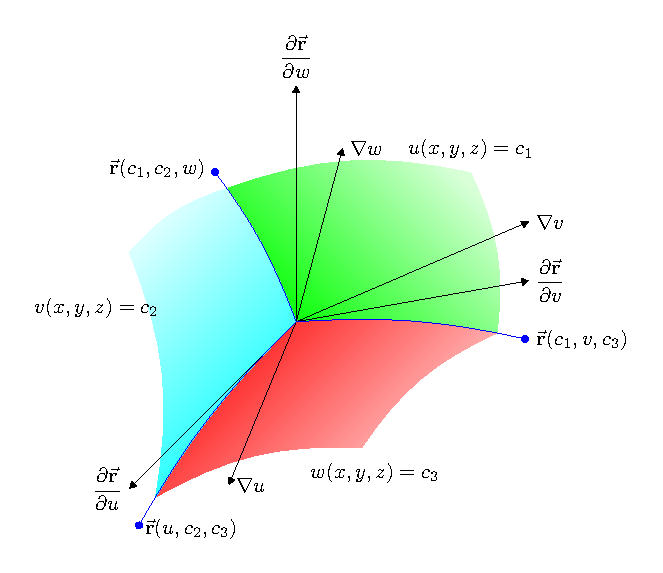
\includegraphics[scale=1.3]{Imagenes/Superficies_Curvas_Coordenadas.eps}
    \caption{Superficies y curvas de coordenadas}
    \label{fig:figura_02_01}
\end{figure}

Considera los vectores:
\begin{align}
\va{E}^{1} = \grad{u}, \hspace{1cm} \va{E}^{2} = \grad{v}, \hspace{1cm} \va{E}^{3} = \grad{w}
\label{eq:ecuacion_02_12}
\end{align}
evaluados en el punto común de intersección $(c_{1}, c_{2}, c_{3})$ de las superficies de coordenadas. El sistema de vectores $(\va{E}^{1}, \va{E}^{2}, \va{E}^{3})$ se puede seleccionar como un sistema de vectores base que son normales a las superficies de coordenadas. Del mismo modo, los vectores
\begin{align}
\va{E}_{1} = \pdv{\va{r}}{u}, \hspace{1cm} \va{E}_{2} = \pdv{\va{r}}{v}, \hspace{1cm} \va{E}_{3} = \pdv{\va{r}}{w}
\label{ec:ecuacion_02_13}
\end{align}
cuando se evalúa en el punto común de intersección $(c_{1}, c_{2}, c_{3})$ forma un sistema de vectores $(\va{E}_{1}, \va{E}_{2}, \va{E}_{3})$ que podemos seleccionar como base. Esta base es un conjunto de vectores tangentes a las curvas de coordenadas. Ahora se demuestra que la base normal $(\va{E}^{1}, \va{E}^{2}, \va{E}^{3})$ y la base tangencial $(\va{E}_{1}, \va{E}_{2}, \va{E}_{3})$ son un conjunto de bases recíprocas.
\par
Recordemos que $\va{r} = x \, \vu{e}_{1} + y \, \vu{e}_{2} + z \, \vu{e}_{3}$ denota el vector de posición de un punto variable. Sustituyendo $x, y, z$ de la ec. (\ref{eq:ecuacion_02_08}) se obtiene:
\begin{align}
\va{r} = \va{r} (u, v, w) = x (u, v, w) \, \vu{e}_{1} + y (u, v, w) \, \vu{e}_{2} + z (u, v, w) \, \vu{e}_{3}
\label{eq:ecuacion_02_14}
\end{align}

Un pequeño cambio en el vector $\va{r}$ se escribe:
\begin{align}
\dd{\va{r}} = \dd{x} \, \vu{e}_{1} + \dd{y} \, \vu{e}_{2} + \dd{z} \, \vu{e}_{3} = \pdv{\va{r}}{u} \dd{u} + \pdv{\va{r}}{v} \dd{v} + \pdv{\va{r}}{w} \dd{w}
\label{eq:ecuacion_02_15} 
\end{align}
donde las derivadas parciales son:
\begin{align}
\begin{aligned}
\pdv{\va{r}}{u} &= \pdv{x}{u} \vu{e}_{1} + \pdv{y}{u} \vu{e}_{2} + \pdv{z}{u} \vu{e}_{3} \\[0.5em] 
\pdv{\va{r}}{v} &= \pdv{x}{v} \vu{e}_{1} + \pdv{y}{v} \vu{e}_{2} + \pdv{z}{v} \vu{e}_{3} \\[0.5em]
\pdv{\va{r}}{w} &= \pdv{x}{w} \vu{e}_{1} + \pdv{y}{w} \vu{e}_{2} + \pdv{z}{w} \vu{e}_{3}
\end{aligned}
\label{eq:ecuacion_02_16}
\end{align}
En términos de las coordenadas $u, v, w$, se puede pensar que este cambio se mueve a lo largo de la diagonal del paralelepípedo que tiene los lados del vector:
\begin{align*}
\pdv{\va{r}}{u} \dd{u}, \hspace{1cm} \pdv{\va{r}}{v} \dd{v}, \hspace{1cm} \pdv{\va{r}}{w} \dd{w}
\end{align*}

Si suponemos que $u = u(x, y, z)$ está definido por la ecuación (\ref{eq:ecuacion_02_09}) y diferenciando esta relación, obtenemos:
\begin{align}
\dd{u} = \pdv{u}{x} \dd{x} + \pdv{u}{y} \dd{y} + \pdv{u}{z} \dd{z}
\label{eq:ecuacion_02_17}
\end{align}

La ecuación (\ref{eq:ecuacion_02_15}) nos permite representar este diferencial de la forma:
\begin{align}
\begin{aligned}
\dd{u} &= \grad{u} \cdot \dd{\va{r}} \\[0.5em]
\dd{u} &= \grad{u} \cdot \left( \pdv{\va{r}}{u} \dd{x} + \pdv{\va{r}}{v} \dd{v} + \pdv{\va{r}}{w} \dd{w} \right) \\[0.5em]
\dd{u} &= \left( \grad{u} \cdot \pdv{\va{r}}{u} \right) \dd{u} + \left( \grad{u} \cdot \pdv{\va{r}}{v} \right) \dd{v} + \left( \grad{u} \cdot \pdv{\va{r}}{w} \right) \dd{w}
\end{aligned}
\label{eq:ecuacion_02_18}
\end{align}
Al comparar términos semejantes en esta última ecuación, encontramos que:
\begin{align}
\va{E}^{1} \cdot \va{E}_{1} = 1, \hspace{1cm} \va{E}^{1} \cdot \va{E}_{2} = 0, \hspace{1cm} \va{E}^{1} \cdot \va{E}_{3} = 0
\label{eq:ecuacion_02_19}
\end{align}

De manera similar, para las otras dos ecuaciones en (\ref{eq:ecuacion_02_09}), las que definen $v = v(x, y, z)$ y $w = w (x, y, z)$, se puede demostrar que:
\begin{align}
\dd{v} &= \left( \grad{v} \cdot \pdv{\va{r}}{u} \right) \dd{u} + \left( \grad{v} \cdot \pdv{\va{r}}{v} \right) \dd{v} + \left( \grad{v} \cdot \pdv{\va{r}}{w} \right) \dd{w}
\label{eq:ecuacion_02_20}
\end{align}
y que:
\begin{align}
\dd{w} &= \left( \grad{w} \cdot \pdv{\va{r}}{u} \right) \dd{u} + \left( \grad{w} \cdot \pdv{\va{r}}{v} \right) \dd{w} + \left( \grad{w} \cdot \pdv{\va{r}}{w} \right) \dd{w}
\label{eq:ecuacion_02_21}
\end{align}
Comparando los términos semejantes en las ecuaciones (\ref{eq:ecuacion_02_20}) y (\ref{eq:ecuacion_02_21}), se tiene que:
\begin{align}
\begin{aligned}
\va{E}^{2} \cdot \va{E}_{1} &= 0, \hspace{1cm} \va{E}^{2} \cdot \va{E}_{2} = 1, \hspace{1cm} \va{E}^{2} \cdot \va{E}_{3} = 0 \\[0.5em]
\va{E}^{3} \cdot \va{E}_{1} &= 0, \hspace{1cm} \va{E}^{3} \cdot \va{E}_{2} = 0, \hspace{1cm} \va{E}^{3} \cdot \va{E}_{3} = 1
\end{aligned}
\label{eq:ecuacion_02_22}
\end{align}
Las ecuaciones (\ref{eq:ecuacion_02_22}) y (\ref{eq:ecuacion_02_19}) nos muestran que los vectores base definidos por las ecuaciones (\ref{eq:ecuacion_02_12}) y (\ref{ec:ecuacion_02_13}) son recíprocos.
\par
Introduciendo la notación:
\begin{align}
(x^{1}, x^{2}, x^{3}) = (u, v, w) \hspace{1.5cm} (y^{1}, y^{2}, y^{3}) = (x, y, z)
\label{eq:ecuacion_02_23}
\end{align}
donde las $x$ denotan las coordenadas generalizadas y las $y$ las coordenadas cartesianas rectangulares, las ecuaciones anteriores se pueden expresar en una forma más concisa con la notación de índices. Por ejemplo, si:
\begin{align}
\begin{aligned}
x^{i} &= x^{i} (x, y, z) = x^{i} (y^{1}, y^{2}, y^{3}), \hspace{0.5cm} \\[0.5em]y^{i} &= y^{i} (u, v, w) = y^{i} (x^{1}, x^{2}, x^{3}), \hspace{1cm} i = 1, 2, 3
\end{aligned}
\label{ec:ecuacion_02_24}
\end{align}
entonces se pueden representar los vectores de base recíproca:
\begin{align}
\va{E}^{i} = \grad{x^{1}}, \hspace{1cm} i = 1, 2, 3
\label{eq:ecuacion_02_25}
\end{align}
y
\begin{align}
\va{E}_{i} = \pdv{\va{r}}{x^{1}}, \hspace{1cm} i = 1, 2, 3
\label{eq:ecuacion_02_26}
\end{align}
Veamos ahora que esas bases de vectores son recíprocas. \hfill \break Notemos que $\va{r} = \va{r} (x^{1}, x^{2}, x^{3})$ con:
\begin{align}
\va{r} = \pdv{\va{r}}{x^{m}} \dd{x^{m}}
\label{eq:ecuacion_02_27}
\end{align}
y en consecuencia:
\begin{align}
\begin{aligned}[b]
\dd{x^{i}} &= \grad{x^{i}} \cdot \dd{\va{r}} = \\[0.5em]
&= \grad{x^{i}} \cdot \pdv{\va{r}}{x^{m}} \dd{x^{m}} = \\[0.5em]
&= \left( \va{E}^{i} \cdot \va{E}_{m} \right) \dd{x^{m}} = \\[0.5em]
&= \delta_{m}{i} \dd{x^{m}}
\end{aligned}
\label{eq:ecuacion_02_28}
\end{align}
Comparando los términos semejantes en esta última ecuación, se tiene el siguiente resultado:
\begin{align*}
\va{E}^{i} \cdot \va{E}_{m} = \delta_{m}^{i}, \hspace{1cm} i = 1, 2, 3
\end{align*}
lo que demuestra que las bases de los vectores son recíprocas.

\section{Escalares, vectores y tensores.}

Los tensores son cantidades que obedecen a ciertas leyes de transformación. Es decir, los escalares, vectores, matrices y matrices de orden superior pueden considerarse componentes de una cantidad tensorial.
\par
Nos interesará saber cómo se representan estos componentes en varios sistemas de coordenadas. Deseamos conocer estas leyes de transformación para poder representar varias leyes físicas en una forma que sea independiente del sistema de coordenadas elegido. Antes de definir diferentes tipos de tensores, examinemos lo que entendemos por transformación de coordenadas.
\par
Las transformaciones de coordenadas del tipo que se encuentran en las ecuaciones () y () se pueden generalizar a dimensiones superiores. Sea $x^{i}, i = 1, 2,\ldots, N$ denotan $N$ variables. Se puede pensar que estas cantidades representan un punto variable cualquiera $(x^{1}, x^{2}, \ldots, x^{N})$ en un espacio $N$ dimensional $V_{N}$. Otro conjunto de $N$ cantidades, llamémosle cantidades con barra: $\overline{x}^{i}, i = 1,2, \ldots, N$, se puede utilizar para representar un punto variable $(\overline{x}^{1}, \overline{x}^{2}, \ldots, \overline{x}^{N})$ en un $N$ espacio dimensional $\overline{V}_{N}$. Cuando las $x$ están relacionadas con las $\overline{x}$ por ecuaciones de la forma:
\begin{align}
x^{i} = x^{i} \, (\overline{x}^{1}, \overline{x}^{2}, \ldots, \overline{x}^{N}), \hspace{1cm} i = 1, 2, \ldots, N
\label{eq:ecuacion_02_30}
\end{align}
entonces se dice que existe una transformación entre las coordenadas $x^{i}$ y $\overline{x}^{i}, i = 1, 2, \ldots, N$. Siempre que las relaciones (\ref{eq:ecuacion_02_30}) sean funcionalmente independientes, univaluadas y posean derivadas parciales tales que el Jacobiano de la transformación:
\begin{align}
J \left( \dfrac{x}{\overline{x}} \right) = J \left( \dfrac{x^{1}, x^{2}, \ldots, x^{N}}{\overline{x}^{1}, \overline{x}^{2}, \ldots, \overline{x}^N} \right) = \mqty|
\displaystyle \pdv{x^{1}}{\overline{x}^{1}} & \displaystyle \pdv{x^{1}}{\overline{x}^{2}} & \ldots & \displaystyle \pdv{x^{1}}{\overline{x}^{N}} \\
\vdots & \vdots & \ldots & \vdots \\
\displaystyle \pdv{x^{N}}{\overline{x}^{1}} & \displaystyle \pdv{x^{N}}{\overline{x}^{2}} & \ldots & \displaystyle \pdv{x^{N}}{\overline{x}^{N}} |
\label{ec:ecuacion_02_31}
\end{align}
es distinto de cero, entonces existes una transformación inversa:
\begin{align}
\overline{x}^{i} = x^{i} (\overline{x}) (x^{1}, x^{2}, \ldots, x^{N}), \hspace{1cm} i = 1, 2, \ldots, N
\label{ec:ecuacion_02_32}
\end{align}
Por brevedad, las ecuaciones de transformación (\ref{eq:ecuacion_02_30}) y (\ref{ec:ecuacion_02_32}) a veces se expresan mediante la notación:
\begin{align}
x^{i} = x^{i} (\overline{x}), \hspace{0.5cm} i = 1, \ldots, N \hspace{0.5cm} \mbox{y} \hspace{0.5cm} \overline{x}^{i} = \overline{x}^{i} (x), \hspace{0.5cm} i =1, \ldots, N
\label{eq:ecuacion_02_33}
\end{align}

Considera una secuencia de transformaciones desde $x$ hasta $\overline{x}$ y luego desde las coordenadas $\overline{x}$ hasta $\overline{\overline{x}}$. Por simplicidad sea $\overline{x} = y$ = y $\overline{\overline{x}} = z$. Si denotamos por $T_{1}, T_{2}$ y $T_{3}$ las transformaciones:
\begin{align*}
T_{1}: y^{i} = y^{i} (x^{1}, \ldots, x^{N}) \hspace{0.3cm} i = 1, \ldots, N \hspace{0.3cm} \mbox{o} \hspace{0.3cm} T_{1} \, x = y \\[0.5em]
T_{2}: z^{i} = z^{i} (y^{1}, \ldots, y^{N}) \hspace{0.3cm} i = 1, \ldots, N \hspace{0.3cm} \mbox{o} \hspace{0.3cm} T_{2} \, y = z
\end{align*}
Entonces, la transformación $T_{3}$ obtenida al sustituir $T_{1}$ en $T_{2}$ se denomina producto de dos transformaciones sucesivas y se escribe:
\begin{align*}
T_{3}: z^{i} &= z^{i} (y^{1} (x^{1}, \ldots, x^{N}), \ldots, y^{N} (x^{1}, \ldots, x^{N})) \hspace{0.3cm} i = 1, \ldots, N \\[0.5em]
\mbox{o} \hspace{0.3cm} T_{3} \, x &= T_{2} \, T_{1} \, x = z
\end{align*}
Esta transformación de producto se denota simbólicamente por $T_{3} = T_{2} \, T_{1}$.
\par
El Jacobiano de la transformación del producto es igual al producto de los Jacobianos asociados con la transformación del producto y $J_{3} = J_{2} \, J_{1}$.

\section{Las transformaciones forman un grupo.}

Un grupo $G$ es un conjunto de elementos no vacíos junto con una ley, para combinar los elementos. Los elementos combinados se indican mediante un producto. Por lo tanto, si $a$ y $b$ son elementos en $G$, no importa cómo se defina la ley para combinar elementos, la combinación de productos se denota $a \, b$. El conjunto $G$ y la ley de combinación forman un grupo si se satisfacen las siguientes propiedades:
\begin{enumerate}[label= (\roman*)]
\item Para todo $a, b \in G$, entonces $a \, b \in G$. Esto se llama propiedad de cerradura.
\item Existe un elemento de identidad $I$ tal que para todo $a \in G$ tenemos que $I \, a = a \, I = a$.
\item Existe un elemento inverso. Es decir, para todo $a \in G$ existe un elemento inverso $a^{-1}$ tal que $a \, a^{-1} = a^{-1} \, a = I$.
\item La ley asociativa se cumple bajo la ley de combinación, así que: $a \, (b \, c) = (a \, b) \,  c$ para todo $a, b, c \in G$.
\end{enumerate}

Por ejemplo, el conjunto de elementos $G = {1, -1, i, -i}$, donde $i^{2} = -1$ junto con la ley de combinación de la multiplicación ordinaria, forma un grupo. Esto se puede ver en la siguiente tabla de multiplicación:
\begin{table}[H]
\centering
\begin{tabular}{| c | c | c | c | c |} \hline
$\times$ & $1$ & $-1$ & $i$ & $-i$ \\ \hline
$1$ & $1$ & $-1$ & $i$ & $-i$ \\ \hline
$-1$ & $-1$ & $1$ & $-i$ & $i$ \\ \hline
$-i$ & $-i$ & $i$ & $1$ & $-1$ \\ \hline
$i$ & $i$ & $-i$ & $-1$ & $1$ \\ \hline
\end{tabular}
\end{table}

El conjunto de todas las transformaciones de coordenadas de la forma encontrada en la ecuación (\ref{eq:ecuacion_02_30}), con Jacobiano diferente de cero, forma un grupo ya que:
\begin{enumerate}[(i)]
\item La transformación del producto, que consta de dos transformaciones sucesivas, pertenece al conjunto de transformaciones. (Cerradura)
\item La transformación de identidad existe en el caso especial de que $\overline{x}$ y $x$ son las mismas coordenadas.
\item La transformación inversa existe porque el Jacobiano de cada transformación individual es diferente de cero.
\item La ley asociativa se satisface en el sentido de que las transformaciones satisfacen la propiedad $T_{3} \, (T_{2} \, T1_{)} = (T_{3} \, T_{2}) \, T_{1}$.
\end{enumerate}
Cuando las ecuaciones de transformación dadas contienen un parámetro, la ley de combinación a menudo se representa como un producto de operadores simbólicos. Por ejemplo, denotamos por $T_{\alpha}$ una transformación de coordenadas que tienen un parámetro $\alpha$. La transformación inversa se puede denotar por $T_{\alpha}^{1}$ y se puede escribir como $T_{\alpha} \, x = \overline{x}$ o $x = T_{\alpha}^{-1} \, \overline{x}$. Dejamos que $T_{\beta}$ denote la misma transformación, pero con un parámetro $\beta$, entonces la propiedad transitiva se expresa simbólicamente por $T_{\alpha} \, T_{\beta} = T_{\gamma}$ donde el producto $T_{\alpha} \, T_{\beta}$ representa el resultado de realizar dos transformaciones sucesivas. La primera transformación de coordenadas usa las ecuaciones de transformación dadas y usa el parámetro $\alpha$ en estas ecuaciones. Esta transformación es seguida por otra transformación de coordenadas usando el mismo conjunto de ecuaciones de transformación, pero esta vez el valor del parámetro es $\beta$. El producto simbólico anterior se usa para demostrar que el resultado de aplicar dos transformaciones sucesivas produce un resultado que es equivalente a realizar una única transformación de coordenadas que tienen el valor del parámetro $\gamma$. Por lo general, entonces se puede establecer alguna relación entre los valores de los parámetros $\alpha, \beta$ y $\gamma$.
\par
En esta notación simbólica, dejamos que $T_\theta$ denote la transformación de identidad. Es decir, usar el valor del parámetro de $\theta$ en el conjunto dado de ecuaciones de transformación produce la transformación de identidad. Entonces, la transformación inversa se puede expresar en forma de encontrar el valor del parámetro $\beta$ tal que $T_{\alpha} \, T_{\beta} = T_{\theta}$.


\section{Sistemas coordenados.}

\subsection{Coordenadas cartesianas.}

A veces es conveniente introducir un sistema de coordenadas cartesiano ortogonal que tenga coordenadas $y^{i}, i = 1, 2,\ldots, N$. Este espacio se denota $E_{N}$ y representa un espacio euclidiano $N$-dimensional. Siempre que las coordenadas independientes generalizadas $x^{i}, i = 1, \ldots, N$ sean funciones de las $y$, de tal manera que estas ecuaciones son funcionalmente independientes, entonces existen ecuaciones de transformación independientes:
\begin{align}
y^{i} = y^{i} (x^{1}, x^{2}, \ldots, x^{N}), \hspace{1cm} i = 1, 2, \ldots, N
\label{eq:ecuacion_02_34}
\end{align}
con el Jacobiano distinto de cero. De manera similar, si hay algún otro conjunto de coordenadas generalizadas, digamos un sistema con barras $\overline{x}^{i}, i = 1, \ldots, N$ donde las $x$ son funciones independientes de las $y$, entonces existirá otro conjunto de ecuaciones de transformación independientes:
\begin{align}
y^{i} = y^{i} (\overline{x}^{1}, \overline{x}^{2}, \ldots, \overline{x}^{N}), \hspace{1cm} i = 1, 2, \ldots, N
\label{eq:ecuacion_02_35}
\end{align}
con Jacobiano diferente de cero. Las transformaciones encontradas en las ecuaciones (\ref{eq:ecuacion_02_34}) y (\ref{eq:ecuacion_02_35}) implican que existen relaciones entre las $x$ y las $\overline{x}$ de la forma (\ref{eq:ecuacion_02_30}) con transformaciones inversas de la forma (\ref{ec:ecuacion_02_32}). Cabe recordar que los conceptos e ideas desarrollados en esta sección se pueden aplicar a un espacio $V_{N}$ de cualquier dimensión finita. Las superficies bidimensionales $(N = 2)$ y los espacios tridimensionales $(N = 3)$ ocuparán la mayor parte de nuestro estudio en el curso. En relatividad, uno debe considerar espacios donde $N = 4$.

\subsection{Coordenadas cilíndricas \texorpdfstring{$(r, \theta, z)$}{(r, q, z)}}

Considera la transformación
\begin{align*}
x = x (r, \theta, z) = r \, \cos \theta \hspace{0.6cm} y = y (r, \theta, z) = r \, \sin \theta \hspace{0.6cm} z = z (r, \theta, z) = z
\end{align*}
de las coordenadas rectangulares $(x, y, z)$ a coordenadas cilíndricas $(r, \theta, z)$, como se muestra en la figura (\ref{fig:figura_02_02}). 
\begin{figure}[H]
    \centering
    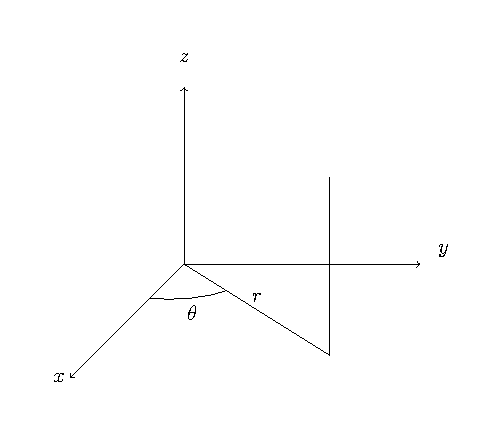
\includegraphics[scale=1]{Imagenes/Sistema_Cilindrico.eps}
    \caption{Coordenadas cilíndricas.}
    \label{fig:figura_02_02}
\end{figure}
Haciendo que:
\begin{align*}
y^{1} = x, \hspace{0.2cm} y^{2} = y, \hspace{0.2cm} y^{3} = z \hspace{0.7cm} x^{1} = r, \hspace{0.2cm} x^{2} = \theta, \hspace{0.2cm} x^{3} = z
\end{align*}
el conjunto de ecuaciones anterior son ejemplos de las ecuaciones de transformación (\ref{eq:ecuacion_02_08}) con $u = r, v = \theta, w = z$ como coordenadas generalizadas.

\subsection{Coordenadas esféricas.}

Considera la transformación:
\begin{align*}
x &= x (\rho, \theta, \phi) = \rho \, \sin \theta \, \cos \phi \\[0.5em]
y &= y (\rho, \theta, \phi) = \rho \, \sin \theta \, \sin \phi \\[0.5em]
z &= z (\rho, \theta, \phi) = \rho \, \cos \theta
\end{align*}
de coordenadas cartesianas $(x, y, z)$ a coordenadas esféricas $(\rho, \theta, \phi)$. Haciendo que:
\begin{align*}
y^{1} = x, \hspace{0.2cm} y^{2} = y, \hspace{0.2cm} y^{3} = z \hspace{0.7cm} x^{1} = \rho, \hspace{0.2cm} x^{2} = \theta, \hspace{0.2cm} x^{3} = \phi
\end{align*}    
el conjunto de ecuaciones anterior tiene la forma que se encuentra en la ecuación (\ref{eq:ecuacion_02_08}) con $u = \rho, v = \theta, w = \phi$ las coordenadas generalizadas. Se podrían colocar barras sobre las $x$ en este ejemplo para distinguir estas coordenadas de las x del ejemplo anterior. Las coordenadas esféricas $(\rho, \theta, \phi)$ muestran en la figura (\ref{fig:figura_02_03}).
\begin{figure}[H]
    \centering
    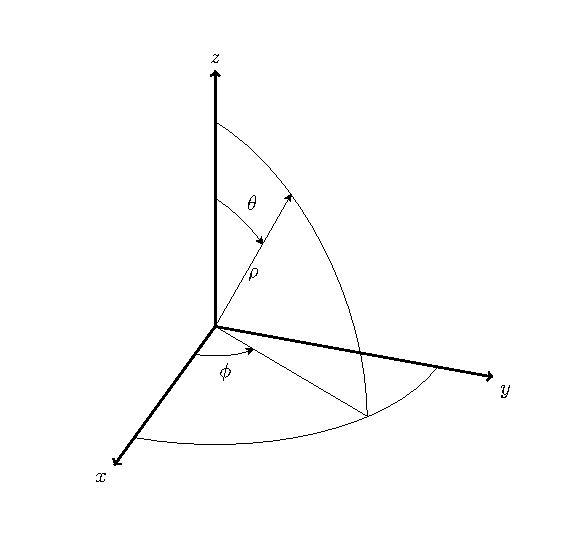
\includegraphics[scale=1]{Imagenes/Sistema_Esferico.eps}
    \caption{Coordenadas esféricas.}
    \label{fig:figura_02_03}
\end{figure}

\section{Funciones escalares e invariancia.}

Ahora estamos en un punto en el que podemos comenzar a definir qué son las cantidades tensoriales. La primera definición es para un \emph{invariante escalar o tensor de orden cero}.

\begin{center}
\noindent\fbox{%
    \parbox{0.8\textwidth}{%
\textbf{Definición: (Campo escalar absoluto)} Supongamos que existe una transformación de coordenadas del tipo (\ref{eq:ecuacion_02_30}) con Jacobiano $J$ distinto de cero. Dejemos que la función escalar:
\begin{align}
f = f (x^{1}, x^{2}, \ldots, x^{N})
\label{eq:ecuacion_02_36}
\end{align}
sea una función de las coordenadas $x^{i}, i = 1, \ldots, N$ en un espacio $V_{N}$. Siempre que exista una función:
\begin{align}
\overline{f} = \overline{f} (\overline{x}^{1}, \overline{x}^{2}, \ldots, \overline{x}^{N})
\label{eq:ecuacion_02_37}
\end{align}
que es función de las coordenadas $\overline{x}^{i}, i = 1, \ldots, N$ tal que $\overline{f} = J^{W} \, f$, entonces $f$ se llama \emph{tensor de rango u orden cero} de peso $W$ en el espacio $V_{N}$. Siempre que $W = 0$, el escalar $f$ se le denomina componente de un campo escalar absoluto y se conoce como un tensor absoluto de rango u orden cero.}%
}
\end{center}
\par
Es decir, un campo escalar absoluto es un objeto invariante en el espacio $V_{N}$ con respecto al grupo de transformaciones de coordenadas. Tiene un solo componente en cada sistema de coordenadas. Para cualquier función escalar del tipo definido por la ecuación (\ref{eq:ecuacion_02_36}), podemos sustituir las ecuaciones de transformación (\ref{eq:ecuacion_02_30}) y obtener:
\begin{align}
f = f (x^{1}, \ldots, x^{N}) = f (x^{1} \, (\overline{x}), \ldots, x^{N} \, (\overline{x}) = \overline{f} = \overline{f} (\overline{x}^{1}, \ldots, \overline{x}^{N})
\label{eq:ecuacion_02_38}
\end{align}

\section{Transformación vectorial, componentes contravariantes.}

En $V_{N}$ considera una curva $C$ definida por el conjunto de ecuaciones paramétricas
\begin{align*}
C: x^{i} = x^{i} (t), \hspace{1cm} i = 1, \ldots, N
\end{align*}
donde $t$ es el parámetro. El vector tangente a la curva $C$ es el vector:
\begin{align*}
\va{T} = \left( \dv{x^{1}}{t}, \dv{x^{2}}{t}, \ldots, \dv{x^{N}}{t} \right)
\end{align*}
En notación de índices, la cual le proporciona el enfoque a los componentes, este vector tangente se escribe como:
\begin{align*}
T^{i} = \dv{x^{i}}{t}, \hspace{1cm} i = 1, \ldots, N
\end{align*}
Para una transformación de coordenadas del tipo definido por la ecuación (\ref{eq:ecuacion_02_30}) con su transformación inversa definida por la ecuación (\ref{ec:ecuacion_02_32}), la curva $C$ se representa en el espacio donde la variables llevan barras por:
\begin{align*}
\overline{x}^{i} = \overline{x}^{i} (x^{1} (t), x^{2} (t), \ldots, x^{N} (t)) = \overline{x}^{i} (t), \hspace{1cm} i = 1, \ldots, N
\end{align*}
con $t$ sin cambios. La tangente a la curva en el sistema de coordenadas con barras está representada por:
\begin{align}
\dv{\overline{x}^{i}}{t} = \pdv{\overline{x}^{i}}{x^{j}} \, \dv{x^{j}}{t}, \hspace{1cm} i = 1, \ldots, N
\label{eq:ecuacion_02_39}
\end{align}

Haciendo $\overline{T}^{i}, i = 1, \ldots, N$, se denotan los componentes de este vector tangente en el sistema de coordenadas barrado, la ecuación (\ref{eq:ecuacion_02_39}) se puede expresar en la forma:
\begin{align}
\overline{T}^{i} = \pdv{\overline{x}^{i}}{x^{j}} \, T_{j}, \hspace{1cm} i, j = 1, \ldots, N
\label{eq:ecuacion_02_40} 
\end{align}

Se dice que esta ecuación define la ley de transformación asociada con un tensor \emph{contravariante absoluto de rango u orden uno}. En el caso $N = 3$ la forma matricial de esta transformación se representa como:
\begin{align}
\mqty(
\overline{T}^{1} \\[1em]
\overline{T}^{2} \\[1em]
\overline{T}^{3}
) = \mqty(
\displaystyle \pdv{\overline{x}^{1}}{x^{1}} & \displaystyle \pdv{\overline{x}^{1}}{x^{2}} & \displaystyle \pdv{\overline{x}^{1}}{x^{3}} \\[1em]
\displaystyle \pdv{\overline{x}^{2}}{x^{1}} & \displaystyle \pdv{\overline{x}^{2}}{x^{2}} & \displaystyle \pdv{\overline{x}^{2}}{x^{3}} \\[1em]
\displaystyle \pdv{\overline{x}^{3}}{x^{1}} & \displaystyle \pdv{\overline{x}^{3}}{x^{2}} & \displaystyle \pdv{\overline{x}^{3}}{x^{3}}
) \, \mqty(
T^{1} \\[1em]
T^{2} \\[1em]
T^{3}
)
\label{eq:ecuacion_02_41}
\end{align}

Una definición más general es:
\begin{center}
    \noindent\fbox{%
        \parbox{0.8\textwidth}{%
\textbf{Definición: (Tensor contravariante)} Siempre que $N$ cantidades $A^{i}$ en un sistema de coordenadas $(x^{1}, \ldots, x^{N})$ estén relacionadas con $N$ cantidades $\overline{A}^{i}$ en un sistema coordenado $(\overline{x}^{1}, \ldots, \overline{x}^{N})$ tal que el Jacobiano $J$ es diferente de cero, entonces si la ley de transformación:
\begin{align*}
\overline{A}^{i} = J^{W} \, \pdv{\overline{x}^{i}}{x^{j}} \, A^{j}
\end{align*}
se satisface, estas cantidades se denominan \emph{componentes de un tensor relativo de rango u orden uno}, con peso $W$. Siempre que $W = 0$, estas cantidades se denominan componentes de un tensor absoluto de rango u orden uno.}
}
\end{center}
\par
Vemos que la ley de transformación anterior satisface las propiedades del grupo que mencionamos anteriormente.

\section{Transformación vectorial, componentes covariantes.}

Considere un invariante escalar $A (x) = \overline{A} (\overline{x})$ la cual en notación abreviada de la ecuación:
\begin{align*}
A (x^{1}, x^{2}, \ldots, x^{N}) = \overline{A} (\overline{x}^{1}, \overline{x}^{2}, \ldots, \overline{x}^{N})
\end{align*}
involucrando la transformación de coordenadas de la ec. (\ref{eq:ecuacion_02_30}). Con la regla de la cadena podemos diferenciar este invariante y encontrar que las componentes del gradiente deben satisfacer:
\begin{align}
\pdv{\overline{A}}{\overline{x}^{i}} = \pdv{A}{x^{j}} \, \pdv{x^{j}}{\overline{x}^{i}}
\label{eq:ecuacion_02_46}
\end{align}

Haciendo que:
\begin{align*}
A_{j} = \pdv{A}{x^{j}} \hspace{0.3cm} \mbox{y} \hspace{0.3cm} \overline{A}_{i} = \pdv{\overline{A}}{\overline{x}^{i}}
\end{align*}
la ecuación (\ref{eq:ecuacion_02_46}) se puede expresar como la ley de transformación:
\begin{align}
\overline{A}_{i} = A_{j} \, \pdv{x^{j}}{\overline{x}^{i}}
\label{eq:ecuacion_02_47}
\end{align}

Ésta es la ley de transformación para un tensor covariante absoluto de rango u orden uno. Una definición más general es:
\begin{center}
    \noindent\fbox{%
        \parbox{0.8\textwidth}{%
\textbf{Definición: (Tensor covariante)} Siempre que $N$ cantidades $A_{i}$ en un sistema de coordenadas $(x^{1}, \ldots, x^{N})$ estén relacionadas con $N$ cantidades $\overline{A}_{i}$ en un sistema de coordenadas $(\overline{x}^{1}, \ldots, \overline{x}^{N})$, con Jacobiano $J$ distinto de cero, de modo que la ley de transformación:
\begin{align}
\overline{A}_{i} = J^{W} \, \pdv{x^{j}}{\overline{x}^{i}} \, A_{j}
\label{eq:ecuacion_02_48}
\end{align}
se satisface, entonces estas cantidades se denominan \emph{componentes de un tensor covariante relativo de rango u orden uno} que tiene un peso de $W$. Siempre que $W = 0$, estas cantidades se denominan componentes de un tensor covariante absoluto de rango u orden uno.}
}
\end{center}
\par
Nuevamente notamos que la transformación anterior satisface las propiedades del grupo. Los \emph{tensores absolutos de rango u orden uno se denominan vectores}, mientras que los \emph{tensores absolutos de rango u orden cero se denominan escalares}.

\section{Tensores de orden superior.}

Hemos demostrado que los tensores de primer orden son cantidades que obedecen a ciertas leyes de transformación. Los tensores de orden superior se definen de manera similar y también satisfacen las propiedades del grupo.
\par
Suponemos que se nos dan transformaciones del tipo ilustrado en las ecuaciones (\ref{eq:ecuacion_02_30}) y (\ref{ec:ecuacion_02_32}) que tienen un solo valor (son univaluadas) y son continuas con el Jacobiano $J$ diferente de cero. Además, las cantidades $x^{i}$ y $\overline{x}^{i}, i = 1, \ldots, n$ representan las coordenadas en dos sistemas de coordenadas cualesquiera. Las siguientes leyes de transformación definen los \emph{tensores de segundo y tercer orden}.
\begin{center}
    \noindent\fbox{%
        \parbox{0.8\textwidth}{%
\textbf{Definición: (Tensor contravariante de segundo orden)}  Siempre que $N$ cantidades al cuadrado $A^{ij}$ en un sistema de coordenadas $(x^{1}, \ldots, x^{N})$ estén relacionadas con $N$ cantidades al cuadrado $\overline{A}^{mn}$ en un sistema coordenado $(\overline{x}^{1}, \ldots, \overline{x}^{N})$ tal que si la ley de transformación:
\begin{align}
\overline{A}^{mn} (\overline{x}) = A^{ij} (x) \, J^{W} \, \pdv{\overline{x}^{m}}{x^{i}} \, \pdv{\overline{x}^{n}}{x^{j}}
\label{eq:ecuacion_02_49}
\end{align}
se satisface, entonces estas cantidades se denominan \emph{componentes de un tensor contravariante relativo de rango u orden dos} con peso $W$. Siempre que $W = 0$, estas cantidades se denominan componentes de un tensor contravariante absoluto de rango u orden dos.}
}
\end{center}

\begin{center}
    \noindent\fbox{%
        \parbox{0.8\textwidth}{%
\textbf{Definición: (Tensor covariante de segundo orden)} Siempre que $N$ cantidades al cuadrado $A_{ij}$ en un sistema de coordenadas $(x^{1}, \ldots, x^{N})$ estén relacionadas con $N$ cantidades al cuadrado $\overline{A}_{mn}$ en un sistema coordenado $(\overline{x}^{1}, \ldots, \overline{x}^{N})$ tal que si la ley de transformación:
\begin{align}
\overline{A}_{mn} (\overline{x}) = A_{ij} (x) \, J^{W} \, \pdv{x^{i}}{\overline{x}^{m}} \, \pdv{x^{j}}{\overline{x}^{n}}
\label{eq:ecuacion_02_50}
\end{align}
se satisface, entonces estas cantidades se denominan \emph{componentes de un tensor covariante relativo de rango u orden dos} con peso $W$. Siempre que $W = 0$, estas cantidades se denominan componentes de un tensor covariante absoluto de rango u orden dos.}
}
\end{center}

\begin{center}
    \noindent\fbox{%
        \parbox{0.8\textwidth}{%
\textbf{Definición: (Tensor mixto de segundo orden)} Siempre que $N$ cantidades al cuadrado $A_{j}^{i}$ en un sistema de coordenadas $(x^{1}, \ldots, x^{N})$ estén relacionadas con $N$ cantidades al cuadrado $\overline{A}_{n}^{m}$ en un sistema coordenado $(\overline{x}^{1}, \ldots, \overline{x}^{N})$ tal que si la ley de transformación:
\begin{align}
\overline{A}_{n}^{m} (\overline{x}) = A_{j}^{i} (x) \, J^{W} \, \pdv{\overline{x}^{m}}{x^{i}} \, \pdv{x^{j}}{\overline{x}^{n}}
\label{eq:ecuacion_02_51}
\end{align}    
se satisface, entonces estas cantidades se denominan \emph{componentes de un tensor mixto relativo de rango u orden dos} con peso $W$. Siempre que $W = 0$, estas cantidades se denominan componentes de un tensor mixto absoluto de rango u orden dos. Es contravariante de orden uno y covariante de orden uno.}
}
\end{center}
Los tensores de orden mayor se definen de manera similar. Por ejemplo, si encontramos que $N$ cantidades al cubo $A_{n p}^{m}$ tales que:
\begin{align}
\overline{A}_{jk}^{i} (\overline{x}) = A_{\alpha \beta}^{\gamma} \, J^{W} \, \pdv{\overline{x}^{i}}{x^{\gamma}} \, \pdv{x^{\alpha}}{\overline{x}^{j}} \, \pdv{x^{\beta}}{\overline{x}^{k}}
\label{eq:ecuacion_02_52}
\end{align}
entonces, este es un tensor relativo mixto de orden tres con peso $W$. Es contravariante de orden uno y covariante de orden dos.

\section{Definición general.}

De manera general, un tensor mixto de orden $(m + n)$:
\begin{align}
T_{j_{1} j_{2} \ldots j_{n}}^{i_{1} i_{2} \ldots i_{m}}
\label{eq:ecuacion_02_53}
\end{align}
es contravariante de orden $m$ y covariante de orden $n$, si obedece la ley de transformación:
\begin{align}
\overline{T}_{j_{1} j_{2} \ldots j_{n}}^{i_{1} i_{2} \ldots i_{m}} = \bigg[ J \left( \dfrac{x}{\overline{x}} \right) \bigg]^{W} \, T_{b_{1} b_{2} \ldots b_{n}}^{a_{1} a_{2} \ldots a_{m}} \, \pdv{\overline{x}^{i_{1}}}{x^{a_{1}}} \, \pdv{\overline{x}^{i_{2}}}{x^{a_{2}}} \, \ldots \, \pdv{\overline{x}^{i_{m}}}{x^{a_{m}}} \cdot \pdv{\overline{x}^{b_{1}}}{\overline{x}^{j_{1}}} \, \pdv{\overline{x}^{b_{2}}}{\overline{x}^{j_{2}}} \, \ldots \, \pdv{\overline{x}^{b_{n}}}{\overline{x}^{j_{n}}}
\label{eq:ecuacion_02_54}
\end{align}
donde:
\begin{align*}
J \left( \dfrac{x}{\overline{x}} \right) = \abs{\pdv{x}{\overline{x}}} = \pdv{(x^{1}, x^{2}, \ldots, x^{N})}{(\overline{x}^{1}, \overline{x}^{2}, \ldots, \overline{x}^{N})}
\end{align*}
es el Jacobiano de la transformación. Cuando $W = 0$, el tensor se llama \emph{tensor absoluto}; de lo contrario, se llama \emph{tensor relativo} de peso $W$.
\par
Aquí se utilizan superíndices para denotar componentes contravariantes y se utilizan subíndices para denotar componentes covariantes. Por lo tanto, si se nos dan las componentes del tensor en un sistema de coordenadas, las componentes de cualquier otro sistema de coordenadas están determinadas por la ley de transformación de la ecuación (\ref{eq:ecuacion_02_54}). En las siguientes partes de estos materiales de lectura, se deben de tratar a todos los tensores como tensores absolutos, a menos que se especifique lo contrario.

\section{Díadas y políadas.}

Tomemos en cuenta que los vectores se pueden representar en \enquote{negritas} con la notación
\begin{align*}
\vb{A} = A_{i} \, \vb{E}^{i}
\end{align*}
Esta notación también se puede generalizar a cantidades tensoriales. Los tensores de orden superior también pueden indicarse con letras en negrita. Por ejemplo, los componentes tensoriales $T_{ij}$ y $B_{ijk}$ se pueden representar en términos de los vectores base 
$\vb{E}^{i}, i = 1, \ldots, N$ utilizando una notación similar a la de la representación de vectores. Por ejemplo:
\begin{align*}
T &= T_{ij} \, \vb{E}^{i} \, \vb{E}^{j} \\[0.5em]
B &= B_{ijk} \, \vb{E}^{i} \, \vb{E}^{j} \, \vb{E}^{k}
\end{align*}
Donde $\vb{T}$ denota un tensor con componentes $T_{ij}$ y $\vb{B}$ denota un tensor con componentes $B_{ijk}$. Las cantidades $\vb{E}^{i} \, \vb{E}^{j}$ se denominan \emph{díadas unitarias} y $\vb{E}^{i} \, \vb{E}^{j} \, \vb{E}^{k}$ se denominan \emph{tríadas unitarias}. No hay signo de multiplicación entre los vectores básicos. Esta notación se llama \emph{notación políada}. Una generalización adicional de esta notación es la representación de un tensor arbitrario utilizando los vectores base y base recíproca en negrita. Por ejemplo, un tensor mixto tendría la representación políada:
\begin{align*}
T = T_{l m \ldots n}^{i j \ldots k} \, \vb{E}_{i} \, \vb{E}_{j} \ldots \vb{E}_{k} \, \vb{E}^{l} \, \vb{E}^{m} \ldots \vb{E}^{n}
\end{align*}
Una diádica está formada por el producto externo o directo de dos vectores. Por ejemplo, el producto externo de los vectores:
\begin{align*}
\vb{a} = a_{1} \, \vb{E}^{1} + a_{2} \, \vb{E}^{2} + a_{3} \, \vb{E}^{3} \hspace{0.3cm} \mbox{y} \hspace{0.3cm} \vb{b} = b_{1} \, \vb{E}^{1} + b_{2} \, \vb{E}^{2} + b_{3} \, \vb{E}^{3}
\end{align*}
está dada por la díada:
\begin{align*}
\vb{a} \, \vb{b} &= a_{1} \, b_{1} \, \vb{E}^{1} \, \vb{E}^{1} + a_{1} \, b_{2} \, \vb{E}^{1} \, \vb{E}^{2} + a_{1} \, b_{3} \, \vb{E}^{1} \, \vb{E}^{3} \\[0.5em]  
&{\quad} a_{2} \, b_{1} \, \vb{E}^{2} \, \vb{E}^{1} + a_{2} \, b_{2} \, \vb{E}^{2} \, \vb{E}^{2} + a_{2} \, b_{3} \, \vb{E}^{2} \, \vb{E}^{3} \\[0.5em]
&{\quad} a_{3} \, b_{1} \, \vb{E}^{3} \, \vb{E}^{1} + a_{3} \, b_{2} \, \vb{E}^{3} \, \vb{E}^{2} + a_{3} \, b_{3} \, \vb{E}^{3} \, \vb{E}^{3}
\end{align*}

En general, una díada se puede representar:
\begin{align*}
\vb{A} = A_{ij} \, \vb{E}^{i} \, \vb{E}^{j} \hspace{1.5cm} i, j = 1, \ldots, N
\end{align*}
donde la convención de suma se está ocupando para los índices repetidos. Los coeficientes $A_{ij}$ se denominan coeficientes de la díada. Cuando los coeficientes se escriben como una matriz $N \times N$, se llama matriz. Cada tensor de segundo orden se puede escribir como una combinación lineal de díadas. Las díadas forman la base de los tensores de segundo orden. Como ilustra el ejemplo anterior, las nueve díadas $\left\{ \vb{E}^{1} \, \vb{E}^{1}, \vb{E}^{1} \, \vb{E}^{2}, \ldots, \vb{E}^{3} \, \vb{E}^{3} \right\}$, asociado con los productos externos de vectores base tridimensionales, constituye una base para el tensor de segundo orden $\vb{A} = \vb{a} \, \vb{b}$ que tiene las componentes $A_{ij} = a_{i} \, b_{j}$ con $i, j = 1, 2, 3$. De manera similar, una tríada tiene la forma:
\begin{align*}
\vb{T} = T_{ijk} \, E^{i} \, E^{j} \, E^{k} \hspace{1cm} \mbox{Suma en índices repetidos}
\end{align*}
donde $i, j, k$ tienen el rango $1, 2, \ldots, N$. El conjunto de productos externos o directos $\left\{ \vb{E}^{i} \, \vb{E}^{j} \, \vb{E}^{k} \right\}$, con $i, j, k = 1, \ldots, N$ constituye una base para todos los tensores de tercer orden. Los componentes tensoriales con sufijos mixtos como $C_{jk}^{i}$ se asocian con la base de la tríada de la forma:
\begin{align*}
\vb{C} = C_{jk}^{i} \, \vb{E}_{i} \, \vb{E}^{j} \, \vb{E}^{k}
\end{align*}
donde $i, j, k$ tienen el rango $1, 2, \ldots, N$. Las díadas están asociadas con el producto externo de dos vectores, mientras que las tríadas, tétradas, $\ldots$ están asociadas con productos externos de orden superior. Estos productos directos o externos de orden superior se denominan políadas.
\par
La notación políada es una generalización de la notación vectorial. El tema de cómo se transforman los componentes de las poliadas entre sistemas de coordenadas es el tema del cálculo de tensores.
\par
En coordenadas cartesianas tenemos que $\vb{E}^{i} = \vb{E}_{i} = \vu{e}_{i}$ y una diádica con componentes llamados díadas se escribe $\vb{A} = A_{ij} \, \vu{e}_{i} \, \vu{e}_{j}$ o como:
\begin{align*}
\vb{A} &= A_{11} \, \vu{e}_{1} \, \vu{e}_{1} + A_{12} \, \vu{e}_{1} \vu{e}_{2} + A_{13} \, \vu{e}_{1} \, \vu{e}_{3} \\[0.5em]  
&{\quad} A_{21} \, \vu{e}_{2} \, \vu{e}_{1} + A_{22} \, \vu{e}_{2} \, \vu{e}_{2} + A_{23} \, \vu{e}_{2} \, \vu{e}_{3} \\[0.5em]
&{\quad} A_{31} \, \vu{e}_{3} \, \vu{e}_{1} + A_{32} \, \vu{e}_{3} \, \vu{e}_{2} + A_{33} \, \vu{e}_{3} \, \vu{e}_{3}    
\end{align*}
donde los términos $\vu{e}_{i} \, \vu{e}_{j}$ se denominan díadas unitarias. Toma en cuenta que una diádica tiene nueve componentes en comparación con un vector que tiene solo tres componentes. La diádica conjugada $\vb{A}_{c}$ se define mediante una transposición de los vectores unitarios en $\vb{A}$, para obtener:
\begin{align*}
\vb{A}_{c} &= A_{11} \, \vu{e}_{1} \, \vu{e}_{1} + A_{12} \, \vu{e}_{2} \vu{e}_{1} + A_{13} \, \vu{e}_{3} \, \vu{e}_{1} \\[0.5em]  
&{\quad} A_{21} \, \vu{e}_{1} \, \vu{e}_{2} + A_{22} \, \vu{e}_{2} \, \vu{e}_{2} + A_{23} \, \vu{e}_{3} \, \vu{e}_{2} \\[0.5em]
&{\quad} A_{31} \, \vu{e}_{1} \, \vu{e}_{3} + A_{32} \, \vu{e}_{2} \, \vu{e}_{3} + A_{33} \, \vu{e}_{3} \, \vu{e}_{3}    
\end{align*}
Si una diádica es igual a su conjugada $\vb{A} = \vb{A}_{c}$, entonces $A_{ij} = A_{ji}$ y la diádica se llama \emph{simétrica}. Si una diádica es igual al negativo de su conjugada $\vb{A} = - \vb{A}_{c}$, entonces $A_{ij} = - A_{ji}$ y la diádica se llama \emph{simétrica sesgada}. Una diádica especial llamada \emph{diádica idéntica o factor idem} que está definida por:
\begin{align*}
J = \vu{e}_{1} \, \vu{e}_{1} + \vu{e}_{2} \, \vu{e}_{2} + \vu{e}_{3} \, \vu{e}_{3}
\end{align*}

Esta diádica tiene la propiedad de que la multiplicación del producto escalar antes o después de la multiplicación de $J$ con un vector $\va{V}$ produce el mismo vector $\va{V}$ Por ejemplo:
\begin{align*}
\va{V} \cdot J &= ( V_{1} \, \vu{e}_{1} + V_{2} \, \vu{e}_{2} + V_{3}  \, \vu{e}_{3} ) \cdot J = \\[0.5em]
&= V_{1} \, \vu{e}_{1} \cdot \, \vu{e}_{1} \, \vu{e}_{1} + V_{2} \, \vu{e}_{2} \cdot \,\vu{e}_{2} \, \vu{e}_{2} + V_{3} \,\vu{e}_{3} \cdot \, \vu{e}_{3} \, \vu{e}_{3} = \\[0.5em]
&= \va{V}
\end{align*}
y
\begin{align*}
J \cdot \va{V} &= J \cdot (V_{1} \, \vu{e}_{1} + V_{2} \, \vu{e}_{2} + V_{3} \, \vu{e}_{3}) = \\[0.5em]
&= V_{1} \, \vu{e}_{1} \, \vu{e}_{1} \cdot \vu{e}_{1} + V_{2} \, \vu{e}_{2} \, \vu{e}_{2} \cdot \vu{e}_{2} + V_{3} \, \vu{e}_{3} \, \vu{e}_{3} \cdot \vu{e}_{3} = \\[0.5em]
&= \va{V}
\end{align*}

Una operación diádica que se usa a menudo en física y química es el producto de doble punto $\va{A} : \va{B}$, donde $\va{A}$ y $\va{B}$ son ambos diádicas. Aquí ambas diádicas se expanden usando la ley distributiva de la multiplicación, y luego cada par de díadas unitarias $\vu{e}_{i} \, \vu{e}_{j} : \vu{e}_{m} \, \vu{e}_{n}$ se combinan de acuerdo con la regla:
\begin{align*}
\vu{e}_{i} \, \vu{e}_{j} : \vu{e}_{m} \, \vu{e}_{n} = (\vu{e}_{i} \cdot \vu{e}_{m}) (\vu{e}_{j} \cdot \vu{e}_{n})
\end{align*}

Por ejemplo, si $\va{A} = A_{ij} \, \vu{e}_{i} \, \vu{e}_{j}$ y $\va{B} = B_{ij} \, \vu{e}_{i} \, \vu{e}_{j}$, entonces el doble producto $\vb{A} : \vb{B}$ se calcula de la siguiente manera:
\begin{align*}
\vb{A} : \vb{B} &= (A_{ij} \, \vu{e}_{i} \, \vu{e}_{j}) : (B_{mn} \, \vu{e}_{m} \, \vu{e}_{n} = A_{ij} \, B_{mn} ( \vu{e}_{i} \, \vu{e}_{j} : \vu{e}_{m} \, \vu{e}_{n}) = \\[0.5em]
&= A_{ij} \, B_{mn} \, \delta_{im} \, \delta_{jn} = \\[0.5em]
&= A_{ij} \, B_{mn} = \\[0.5em]
&= A_{11} \, B_{11} + A_{12} \, B_{12} + A_{13} \, B_{13} + \\[0.5em] 
&+ A_{21} \, B_{21} + A_{22} \, B_{22} + A_{23} \, B_{23} + \\[0.5em] 
&+ A_{31} \, B_{31} + A_{32} \, B_{32} + A_{33} \, B_{33} 
\end{align*}
Cuando se opera con díadas, tríadas y políadas, hay un orden definido en la forma en que se representan los vectores y los componentes de la políada. Por ejemplo, para $\va{A} = A_{i} \, \vu{e}_{i}$ y $\va{B} = B_{i} \, \vu{e}_{i}$ vectores con producto externo:
\begin{align*}
\va{A} \, \va{B} = A_{m} \, B_{n} \, \vu{e}_{m} \, \vu{e}_{n} = \phi
\end{align*}
se produce la diádica $\phi$ con componentes $A_{m} \, B_{n}$. En comparación, el producto exterior:
\begin{align*}
\va{B} \, \va{A} = B_{m} \, A_{n} \, \vu{e}_{m} \, \vu{e}_{n} = \psi
\end{align*}
produce la díadica $\psi$ con componentes $B_{m} \, A_{n}$. Esto es:
\begin{align*}
\phi &= \va{A} \, \va{B} =  A_{1} \, B_{1} \, \vu{e}_{1} \, \vu{e}_{1} + A_{1} \, B_{2} \, \vu{e}_{1} \, \vu{e}_{2} + A_{1} \, B_{3} \, \vu{e}_{1} \, \vu{e}_{3} \\[0.5em]
&{\quad} A_{2} \, B_{1} \, \vu{e}_{2} \, \vu{e}_{1} + A_{2} \, B_{2} \, \vu{e}_{2} \, \vu{e}_{2} + A_{2} \, B_{3} \, \vu{e}_{2} \, \vu{e}_{3} \\[0.5em]
&{\quad} A_{3} \, B_{1} \, \vu{e}_{3} \, \vu{e}_{1} + A_{3} \, B_{2} \, \vu{e}_{3} \, \vu{e}_{2} + A_{3} \, B_{3} \, \vu{e}_{3} \, \vu{e}_{3}
\end{align*}
y
\begin{align*}
\psi &= \va{B} \, \va{A} = B_{1} \, A_{1} \, \vu{e}_{1} \, \vu{e}_{1} + B_{1} \, A_{2} \, \vu{e}_{1} \, \vu{e}_{2} + B_{1} \, A_{3} \, \vu{e}_{1} \, \vu{e}_{3} \\[0.5em]
&{\quad} B_{2} \, A_{1} \, \vu{e}_{2} \, \vu{e}_{1} + B_{2} \, A_{2} \, \vu{e}_{2} \, \vu{e}_{2} + B_{2} \, A_{3} \, \vu{e}_{2} \, \vu{e}_{3} \\[0.5em]
&{\quad} B_{3} \, A_{1} \, \vu{e}_{3} \, \vu{e}_{1} + B_{3} \, A_{2} \, \vu{e}_{3} \, \vu{e}_{2} + B_{3} \, A_{3} \, \vu{e}_{3} \, \vu{e}_{3}
\end{align*}
son diádicas distintas.
\par
El producto escalar de una diádica con un vector $\va{C}$ se define por la pre y post multiplicación como:
\begin{align*}
\phi \cdot \va{C} &= \va{A} \, \va{B} \cdot \va{C} = \va{A} \, (\va{B} \cdot \va{C}) \\[0.5em]
\va{C} \cdot \phi &= \va{C} \cdot \va{A} \, \va{B} = (\va{C} \cdot \va{A}) \, \va{B}
\end{align*}
Estos productos en general, no son iguales.
\end{document}